\documentclass[oneside,a4paper,final,14pt]{article}

\usepackage{extsizes}
\usepackage{cmap}

%%% Работа с русским языком
\usepackage[english,russian]{babel}   %% загружает пакет многоязыковой вёрстки
\usepackage{fontspec}      %% подготавливает загрузку шрифтов Open Type, True Type и др.
\defaultfontfeatures{Ligatures={TeX},Renderer=Basic}  %% свойства шрифтов по умолчанию
\setmainfont[Ligatures={TeX,Historic}]{Times New Roman} %% задаёт основной шрифт документа
\setsansfont{Comic Sans MS}                    %% задаёт шрифт без засечек
\setmonofont{Courier New}
\usepackage{indentfirst}
\setlength\parindent{10ex}
\frenchspacing

\usepackage{mathtext}
\usepackage{amsmath,amssymb,amsthm,amsfonts,mathtools}
\usepackage{icomma}
\usepackage{etoolbox}

\usepackage{geometry}
  \geometry{top=15mm}
  \geometry{bottom=15mm}
  \geometry{left=15mm}
  \geometry{right=15mm}

\usepackage{fancyhdr}
  \pagestyle{fancy}
  \renewcommand{\headrulewidth}{0pt}
  %\lfoot{Left bottom}
   \lhead{ }
   \chead{ }
   \rhead{ }
   \cfoot{ }
   \rfoot{\thepage}
  
\usepackage{setspace} % Интерлиньяж
\onehalfspacing % 1.5 интервал

\usepackage{lastpage}

\usepackage{multicol}
\usepackage{array}

\usepackage[noend]{algorithmic}
\usepackage{color}

\usepackage{titlesec}
\titleformat{\section}{\normalsize}{\thesection}{1em}{}
\titlespacing{\section}{\parindent}{*4}{*4}

\usepackage{listings}

\usepackage{graphicx}

\begin{document}
	
\thispagestyle{empty}
\begin{center}
МИНОБРНАУКИ РОССИИ

Федеральное государственное бюджетное образовательное учреждение 

высшего профессионального образования

<<Пензенский государственный технологический университет>>
(ПензГТУ)

\vspace{36pt}

Факультет информационных и образовательных технологий

Кафедра <<Информационные технологии и системы>>

Дисциплина <<Языки программирования>>

\vspace{36pt}

К\,У\,Р\,С\,О\,В\,А\,Я Р\,А\,Б\,О\,Т\,А

на тему: <<Разработка программы сопровождения базы данных на языке ANSI C>>

(предметная область – <<Склад>>)

\vspace{72pt}

ПОЯСНИТЕЛЬНАЯ ЗАПИСКА

ПензГТУ 3.230400.4.ПЗ

\vspace{72pt}

\parbox{12cm}{
Выполнил: студент гр. 14ИС1ба Иванов И.И.

Проверил: ст. преподаватель каф. ИТС Володин К.И.

Работа защищена с оценкой:~\hrulefill
}

\vfill

Пенза 2014
\end{center}

%\newpage
%\tableofcontents

\newpage
\section{Регрессия. Регрессионная модель. Основные понятия}

Регрессионная модель
\[
y=f(x,b)+\varepsilon, ~E(\varepsilon)=0,
\]

где $b$ — параметры модели, $\varepsilon$ — случайная ошибка модели, называется линейной регрессией, если функция регрессии $f(x,b)$ имеет вид
\begin{equation}
f(x,b)=b_0+b_1 x_1+b_2 x_2+\ldots+b_k x_k,
\end{equation}

где $b_j$ — параметры (коэффициенты) регрессии, $x_j$ — регрессоры (факторы модели), $k$ — количество факторов модели.

Коэффициенты линейной регрессии показывают скорость изменения зависимой переменной по данному фактору, при фиксированных остальных факторах (в линейной модели эта скорость постоянна):
\begin{equation}
\forall j ~b_j=\frac {\partial f}{\partial x_j}=const
\end{equation}

Параметр $b_0$, при котором нет факторов, называют часто константой. Формально — это значение функции при нулевом значении всех факторов. Для аналитических целей удобно считать, что константа — это параметр при «факторе», равном 1 (или другой произвольной постоянной, поэтому константой называют также и этот «фактор»). В таком случае, если перенумеровать факторы и параметры исходной модели с учетом этого (оставив обозначение общего количества факторов — $k$), то линейную функцию регрессии можно записать в следующем виде, формально не содержащем константу:
$$f(x,b)=b_1 x_1 + b_2 x_2 + \ldots + b_k x_k=\sum^k_{j=1}b_j x_j=x^Tb,$$

где $x^T=(x_1,x_2,\ldots,x_k)$ — вектор регрессоров, $b=(b_1,b_2, \ldots,b_k)^T$ — вектор-столбец параметров (коэффициентов).

Линейная модель может быть как с константой, так и без константы. Тогда в этом представлении первый фактор либо равен единице, либо является обычным фактором соответственно.

\newpage

\section{Пример построения регрессии по данным}
\vspace{12pt}

Это пример построения регрессии по данным. Это пример построения регрессии по данным. Это пример построения регрессии по данным. Это пример построения регрессии по данным.

\begin{center}
  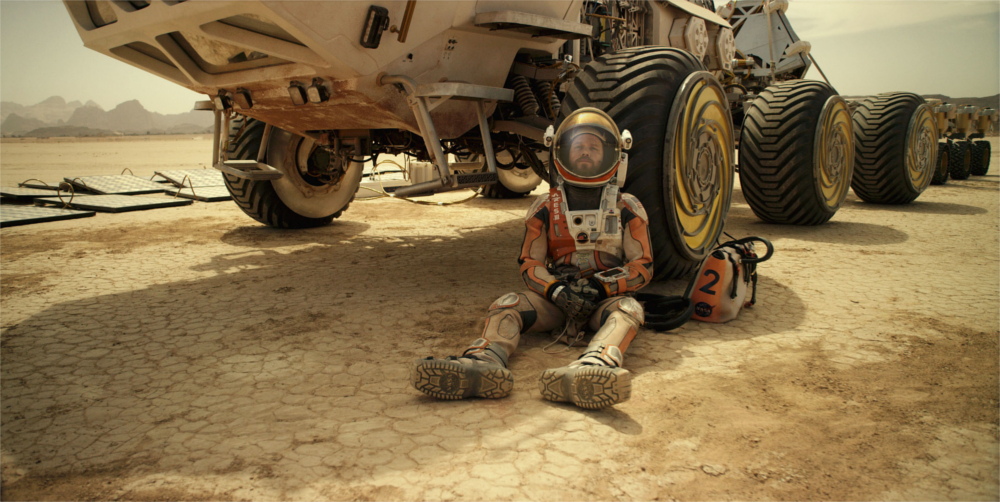
\includegraphics[scale=1.0]{images/rest.jpg}\\
  Рисунок 1 - Это рисунок
\end{center}
\vspace{-12pt}

Это пример построения регрессии по данным. Это пример построения регрессии по данным. Это пример построения регрессии по данным. Это пример построения регрессии по данным.

%% Подставим 






\end{document}
